\documentclass[twoside]{book}

% Packages required by doxygen
\usepackage{fixltx2e}
\usepackage{calc}
\usepackage{doxygen}
\usepackage{graphicx}
\usepackage[utf8]{inputenc}
\usepackage{makeidx}
\usepackage{multicol}
\usepackage{multirow}
\PassOptionsToPackage{warn}{textcomp}
\usepackage{textcomp}
\usepackage[nointegrals]{wasysym}
\usepackage[table]{xcolor}

% Font selection
\usepackage[T1]{fontenc}
\usepackage{mathptmx}
\usepackage[scaled=.90]{helvet}
\usepackage{courier}
\usepackage{amssymb}
\usepackage{sectsty}
\renewcommand{\familydefault}{\sfdefault}
\allsectionsfont{%
  \fontseries{bc}\selectfont%
  \color{darkgray}%
}
\renewcommand{\DoxyLabelFont}{%
  \fontseries{bc}\selectfont%
  \color{darkgray}%
}
\newcommand{\+}{\discretionary{\mbox{\scriptsize$\hookleftarrow$}}{}{}}

% Page & text layout
\usepackage{geometry}
\geometry{%
  a4paper,%
  top=2.5cm,%
  bottom=2.5cm,%
  left=2.5cm,%
  right=2.5cm%
}
\tolerance=750
\hfuzz=15pt
\hbadness=750
\setlength{\emergencystretch}{15pt}
\setlength{\parindent}{0cm}
\setlength{\parskip}{0.2cm}
\makeatletter
\renewcommand{\paragraph}{%
  \@startsection{paragraph}{4}{0ex}{-1.0ex}{1.0ex}{%
    \normalfont\normalsize\bfseries\SS@parafont%
  }%
}
\renewcommand{\subparagraph}{%
  \@startsection{subparagraph}{5}{0ex}{-1.0ex}{1.0ex}{%
    \normalfont\normalsize\bfseries\SS@subparafont%
  }%
}
\makeatother

% Headers & footers
\usepackage{fancyhdr}
\pagestyle{fancyplain}
\fancyhead[LE]{\fancyplain{}{\bfseries\thepage}}
\fancyhead[CE]{\fancyplain{}{}}
\fancyhead[RE]{\fancyplain{}{\bfseries\leftmark}}
\fancyhead[LO]{\fancyplain{}{\bfseries\rightmark}}
\fancyhead[CO]{\fancyplain{}{}}
\fancyhead[RO]{\fancyplain{}{\bfseries\thepage}}
\fancyfoot[LE]{\fancyplain{}{}}
\fancyfoot[CE]{\fancyplain{}{}}
\fancyfoot[RE]{\fancyplain{}{\bfseries\scriptsize Generated on Tue Aug 29 2017 15\+:44\+:16 for Lab 0 by Doxygen }}
\fancyfoot[LO]{\fancyplain{}{\bfseries\scriptsize Generated on Tue Aug 29 2017 15\+:44\+:16 for Lab 0 by Doxygen }}
\fancyfoot[CO]{\fancyplain{}{}}
\fancyfoot[RO]{\fancyplain{}{}}
\renewcommand{\footrulewidth}{0.4pt}
\renewcommand{\chaptermark}[1]{%
  \markboth{#1}{}%
}
\renewcommand{\sectionmark}[1]{%
  \markright{\thesection\ #1}%
}

% Indices & bibliography
\usepackage{natbib}
\usepackage[titles]{tocloft}
\setcounter{tocdepth}{3}
\setcounter{secnumdepth}{5}
\makeindex

% Hyperlinks (required, but should be loaded last)
\usepackage{ifpdf}
\ifpdf
  \usepackage[pdftex,pagebackref=true]{hyperref}
\else
  \usepackage[ps2pdf,pagebackref=true]{hyperref}
\fi
\hypersetup{%
  colorlinks=true,%
  linkcolor=blue,%
  citecolor=blue,%
  unicode%
}

% Custom commands
\newcommand{\clearemptydoublepage}{%
  \newpage{\pagestyle{empty}\cleardoublepage}%
}


%===== C O N T E N T S =====

\begin{document}

% Titlepage & ToC
\hypersetup{pageanchor=false,
             bookmarks=true,
             bookmarksnumbered=true,
             pdfencoding=unicode
            }
\pagenumbering{roman}
\begin{titlepage}
\vspace*{7cm}
\begin{center}%
{\Large Lab 0 }\\
\vspace*{1cm}
{\large Generated by Doxygen 1.8.8}\\
\vspace*{0.5cm}
{\small Tue Aug 29 2017 15:44:16}\\
\end{center}
\end{titlepage}
\clearemptydoublepage
\tableofcontents
\clearemptydoublepage
\pagenumbering{arabic}
\hypersetup{pageanchor=true}

%--- Begin generated contents ---
\chapter{Box Session Information}
\label{Virtual}
\hypertarget{Virtual}{}
 
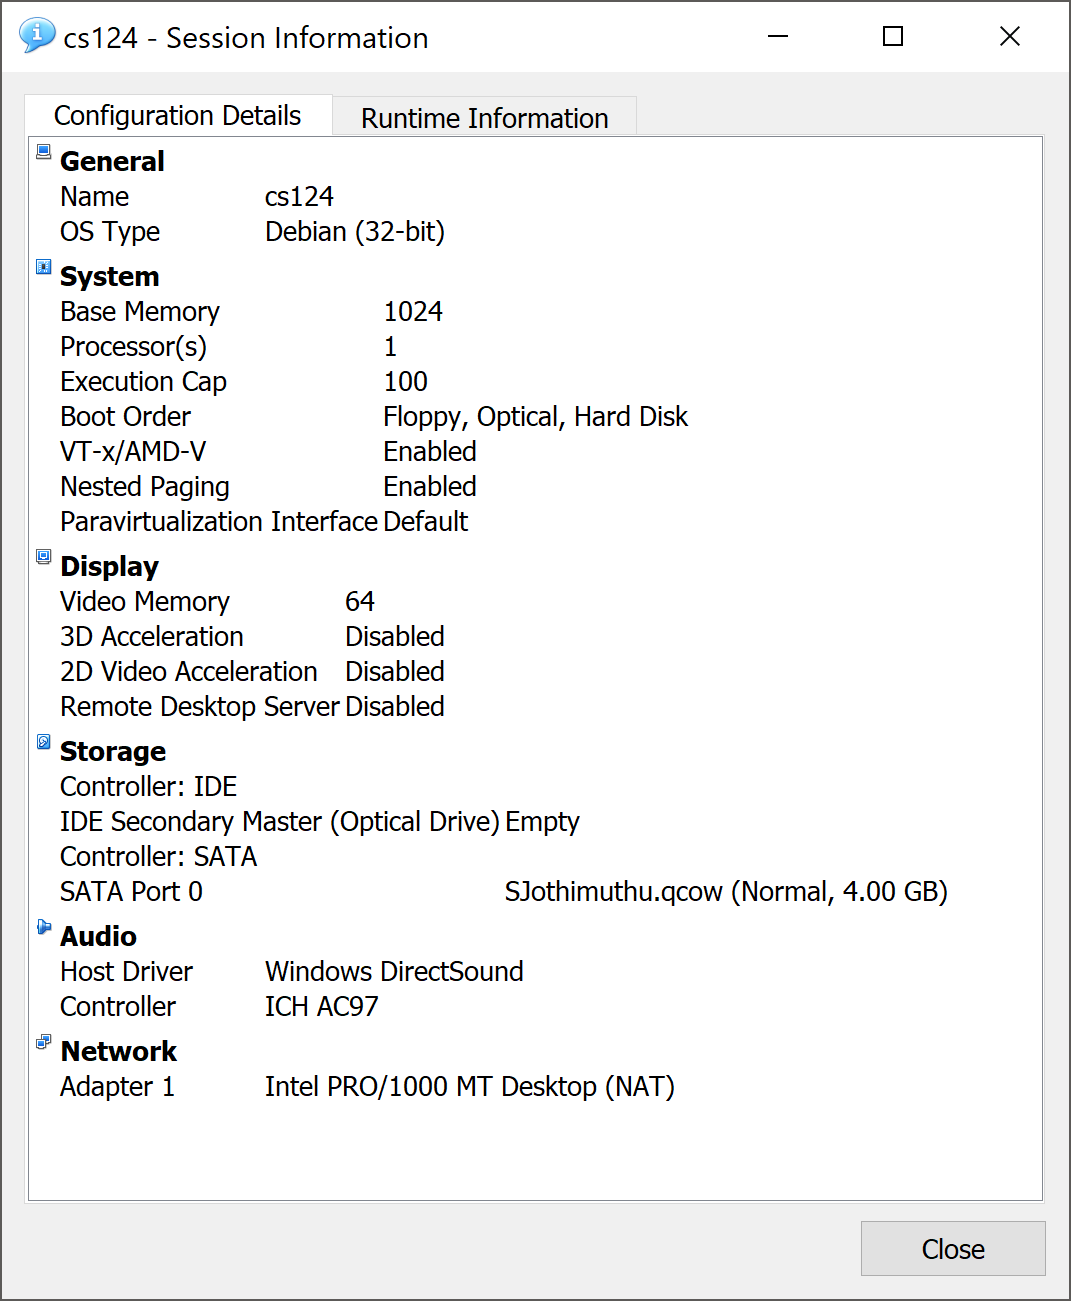
\includegraphics{../config124.png}
 
\chapter{File Index}
\subsection{File List}
Here is a list of all files with brief descriptions\+:\begin{DoxyCompactList}
\item\contentsline{section}{\hyperlink{addWords_8cpp}{add\+Words.\+cpp} }{\pageref{addWords_8cpp}}{}
\item\contentsline{section}{\hyperlink{foundWord_8cpp}{found\+Word.\+cpp} }{\pageref{foundWord_8cpp}}{}
\item\contentsline{section}{\hyperlink{lab_8cpp}{lab.\+cpp} }{\pageref{lab_8cpp}}{}
\item\contentsline{section}{\hyperlink{lab_8h}{lab.\+h} }{\pageref{lab_8h}}{}
\item\contentsline{section}{\hyperlink{loadDictionary_8cpp}{load\+Dictionary.\+cpp} }{\pageref{loadDictionary_8cpp}}{}
\item\contentsline{section}{\hyperlink{main_8cpp}{main.\+cpp} }{\pageref{main_8cpp}}{}
\end{DoxyCompactList}

\chapter{File Documentation}
\hypertarget{fig1_8dox}{\section{fig1.\+dox File Reference}
\label{fig1_8dox}\index{fig1.\+dox@{fig1.\+dox}}
}

\hypertarget{main_8cpp}{\subsection{main.\+cpp File Reference}
\label{main_8cpp}\index{main.\+cpp@{main.\+cpp}}
}
{\ttfamily \#include \char`\"{}lab.\+h\char`\"{}}\\*
Include dependency graph for main.\+cpp\+:\nopagebreak
\begin{figure}[H]
\begin{center}
\leavevmode
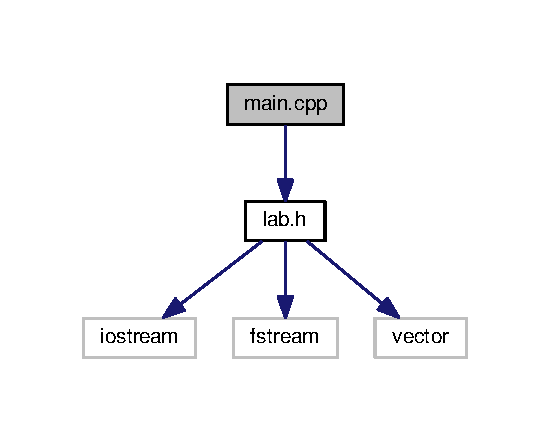
\includegraphics[width=264pt]{main_8cpp__incl}
\end{center}
\end{figure}
\subsubsection*{Functions}
\begin{DoxyCompactItemize}
\item 
int \hyperlink{main_8cpp_ae66f6b31b5ad750f1fe042a706a4e3d4}{main} ()
\end{DoxyCompactItemize}


\subsubsection{Function Documentation}
\hypertarget{main_8cpp_ae66f6b31b5ad750f1fe042a706a4e3d4}{\index{main.\+cpp@{main.\+cpp}!main@{main}}
\index{main@{main}!main.\+cpp@{main.\+cpp}}
\paragraph[{main}]{\setlength{\rightskip}{0pt plus 5cm}int main (
\begin{DoxyParamCaption}
{}
\end{DoxyParamCaption}
)}}\label{main_8cpp_ae66f6b31b5ad750f1fe042a706a4e3d4}
This is main function of the project. Contains the three fucntions (loaddictionary, foundwords, addwords) See comments for better understanding 
\begin{DoxyCode}
11 \{
12     vector<Entry> dict;
13     \textcolor{keywordtype}{string} word; \textcolor{comment}{// user inputs word}
14     \textcolor{keywordtype}{string} translation; \textcolor{comment}{// outputs translation}
15     \textcolor{keywordtype}{bool} ok, quit;
16     
17     ok = \hyperlink{lab_8h_ac18625e34f66c3bc052e07dfb0d3d219}{loaddictionary}(\textcolor{stringliteral}{"dict.dat"}, dict);
18     \textcolor{keywordflow}{if} (!ok) \{
19         cout << \textcolor{stringliteral}{" **** Cannot load Dictionary ***** \(\backslash\)n"};
20         \textcolor{keywordflow}{return} 1; \textcolor{comment}{//ERROR}
21     \}
22     
23     
24     \textcolor{keywordtype}{string} line;
25     
26  ifstream inpfile(\textcolor{stringliteral}{"dict.dat"}); \textcolor{comment}{//opening file again so that once updated }
27     \textcolor{keywordflow}{if} (!inpfile) \textcolor{keywordflow}{return} \textcolor{keyword}{false}; \textcolor{comment}{//the new information can be called without restarting the program}
28     
29     getline(inpfile, line);
30     cout << line << endl;
31     cout << \textcolor{stringliteral}{"Program by Samuel Jothimuthu"} <<endl;
32 
33     quit = \textcolor{keyword}{false};
34     \textcolor{keywordflow}{while} (!quit) \{ \textcolor{comment}{//iteration control structure}
35         \hyperlink{lab_8h_ac18625e34f66c3bc052e07dfb0d3d219}{loaddictionary}(\textcolor{stringliteral}{"dict.dat"}, dict);
36 
37         \textcolor{keywordtype}{string} choice; \textcolor{comment}{//simple choice of yes or no }
38         \textcolor{keywordtype}{string} newtran; \textcolor{comment}{//new translation for word user enters}
39         \textcolor{keywordtype}{string} inputstring; \textcolor{comment}{// the full string that will be appened to the file "dict.dat"}
40         cout << \textcolor{stringliteral}{"Enter a word or 'q' to quit ==> "};
41         cin >> word;
42         cin.ignore(80, \textcolor{charliteral}{'\(\backslash\)n'}); \textcolor{comment}{//this allows the console argument to execute but skipping the line}
43         \textcolor{keywordflow}{if} (word == \textcolor{stringliteral}{"q"}) 
44             quit = \textcolor{keyword}{true};
45         \textcolor{keywordflow}{else} \textcolor{keywordflow}{if} (\hyperlink{foundWord_8cpp_ae41eba27837d0aeea84fb5c6824388db}{foundword}( dict, word, translation)) \textcolor{comment}{//function must return true}
46             cout << translation << \textcolor{stringliteral}{"\(\backslash\)n\(\backslash\)n"};
47         \textcolor{keywordflow}{else} \textcolor{comment}{//The selection control structure}
48            \{ cout << word << \textcolor{stringliteral}{" --not in the dictionary. \(\backslash\)n Would you like to add it? (y/n)\(\backslash\)n"};
49             cin >> choice;
50             \textcolor{keywordflow}{if} (choice == \textcolor{stringliteral}{"y"}) \{ \textcolor{comment}{//any other input does not work. }
51                 cout << \textcolor{stringliteral}{"What is the Italian translation for "} << word << \textcolor{stringliteral}{"?"} << endl;
52                 cin >> newtran;
53                 inputstring = word + \textcolor{stringliteral}{"\(\backslash\)t"} + newtran; \textcolor{comment}{// this builds the full string that the program can
       then call upon.}
54                 \hyperlink{addWords_8cpp_ab5aa985d3bd8d2b89a2d5f35f38fb868}{addwords}(\textcolor{stringliteral}{"dict.dat"}, inputstring); \textcolor{comment}{//runs the addwords function, adding it into the
       file.}
55                 \}
56         \}
57         \}
58         \textcolor{keywordflow}{return} 0;
59     \}
\end{DoxyCode}

%--- End generated contents ---

% Index
\newpage
\phantomsection
\addcontentsline{toc}{chapter}{Index}
\printindex

\end{document}
